%%%%%%%%%%%%%%%%%%%%%%%%%%%%%%%%%%%%%%%%%
% Beamer Presentation
% LaTeX Template
% Version 1.0 (10/11/12)
%
% This template has been downloaded from:
% http://www.LaTeXTemplates.com
%
% License:
% CC BY-NC-SA 3.0 (http://creativecommons.org/licenses/by-nc-sa/3.0/)
%
%%%%%%%%%%%%%%%%%%%%%%%%%%%%%%%%%%%%%%%%%

%----------------------------------------------------------------------------------------
%	PACKAGES AND THEMES
%----------------------------------------------------------------------------------------

\documentclass{beamer}

\mode<presentation> {

% The Beamer class comes with a number of default slide themes
% which change the colors and layouts of slides. Below this is a list
% of all the themes, uncomment each in turn to see what they look like.

%\usetheme{default}
%\usetheme{AnnArbor}
%\usetheme{Antibes}
%\usetheme{Bergen}
%\usetheme{Berkeley}
%\usetheme{Berlin}
%\usetheme{Boadilla}
%\usetheme{CambridgeUS}
%\usetheme{Copenhagen}
%\usetheme{Darmstadt}
%\usetheme{Dresden}
%\usetheme{Frankfurt}
%\usetheme{Goettingen}
%\usetheme{Hannover}
%\usetheme{Ilmenau}
%\usetheme{JuanLesPins}
%\usetheme{Luebeck}
\usetheme{Madrid}
%\usetheme{Malmoe}
%\usetheme{Marburg}
%\usetheme{Montpellier}
%\usetheme{PaloAlto}
%\usetheme{Pittsburgh}
%\usetheme{Rochester}
%\usetheme{Singapore}
%\usetheme{Szeged}
%\usetheme{Warsaw}

% As well as themes, the Beamer class has a number of color themes
% for any slide theme. Uncomment each of these in turn to see how it
% changes the colors of your current slide theme.

%\usecolortheme{albatross}
%\usecolortheme{beaver}
%\usecolortheme{beetle}
%\usecolortheme{crane}
%\usecolortheme{dolphin}
%\usecolortheme{dove}
%\usecolortheme{fly}
%\usecolortheme{lily}
%\usecolortheme{orchid}
%\usecolortheme{rose}
%\usecolortheme{seagull}
%\usecolortheme{seahorse}
%\usecolortheme{whale}
%\usecolortheme{wolverine}

%\setbeamertemplate{footline} % To remove the footer line in all slides uncomment this line
%\setbeamertemplate{footline}[page number] % To replace the footer line in all slides with a simple slide count uncomment this line

%\setbeamertemplate{navigation symbols}{} % To remove the navigation symbols from the bottom of all slides uncomment this line
}

\usepackage{graphicx} % Allows including images
\usepackage{booktabs} % Allows the use of \toprule, \midrule and \bottomrule in tables
\usepackage{animate}

%----------------------------------------------------------------------------------------
%	TITLE PAGE
%----------------------------------------------------------------------------------------

\title[Devices for Biological Systems]{Devices for Biological Systems: On-Chip Horizontal Gene Transfer and 3D-Printed Microfluidic Applications} % The short title appears at the bottom of every slide, the full title is only on the title page

\author{Martin Brennan} % Your name
\institute[UIC] % Your institution as it will appear on the bottom of every slide, may be shorthand to save space
{
University of Illinois at Chicago \\ % Your institution for the title page
\medskip
\textit{mbrenn3@uic.edu} % Your email address
}
\date{December 10, 2015} % Date, can be changed to a custom date

\begin{document}

\begin{frame}
\titlepage % Print the title page as the first slide
\end{frame}

\begin{frame}
\frametitle{Overview} % Table of contents slide, comment this block out to remove it
\tableofcontents % Throughout your presentation, if you choose to use \section{} and \subsection{} commands, these will automatically be printed on this slide as an overview of your presentation
\end{frame}

%----------------------------------------------------------------------------------------
%	PRESENTATION SLIDES
%----------------------------------------------------------------------------------------

%------------------------------------------------
\section{Introduction of Microfluidics and applications to biological research} % Sections can be created in order to organize your presentation into discrete blocks, all sections and subsections are automatically printed in the table of contents as an overview of the talk
%------------------------------------------------

\begin{frame}{Microfluidics}
\begin{columns}[c] % The "c" option specifies centered vertical alignment while the "t" option is used for top vertical alignment
\column{.5\textwidth} % Left column and width
%\textbf{Heading}
\begin{figure}
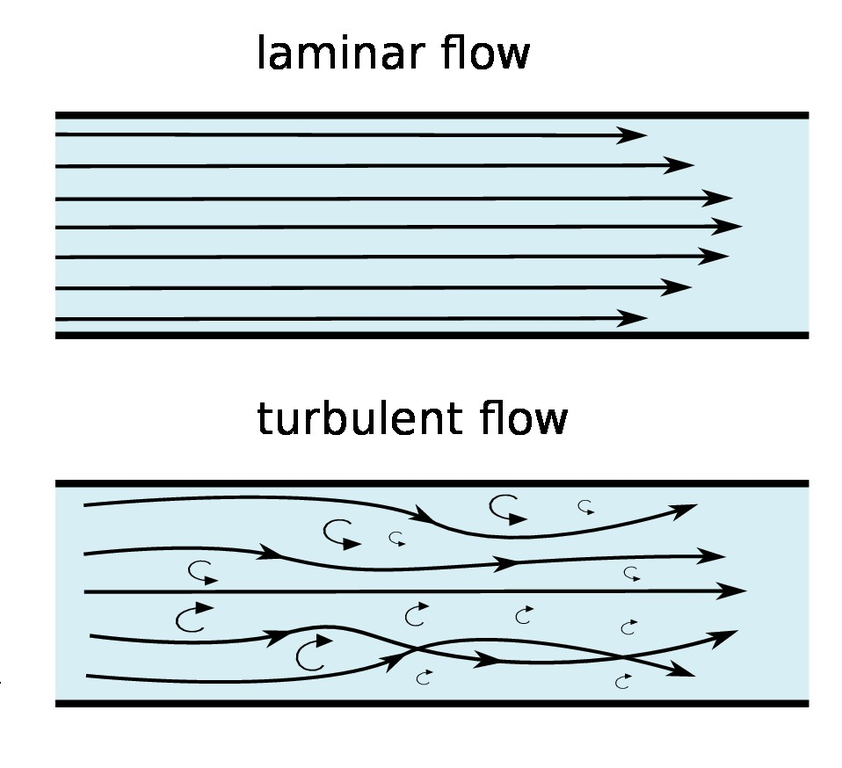
\includegraphics[width=0.6\linewidth]{images/laminar-vs-turbulent-flow.png}\\
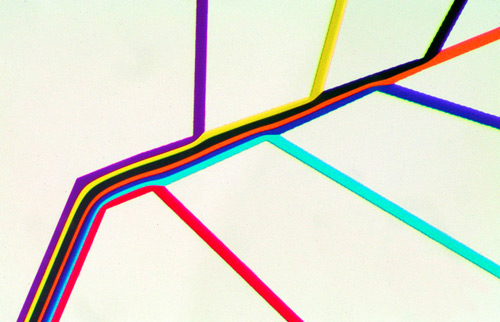
\includegraphics[width=0.6\linewidth]{images/laminar-flow.jpg}\\
\hspace*{11pt}\hbox{\scriptsize \thinspace{\tiny\itshape P.J.A. Kenis et al. Science 285 (1999): 83-85.}}

%culture and monioring of bacteria cultures hundreds of hours
\end{figure}
\column{.5\textwidth} % Right column and width
\begin{figure}
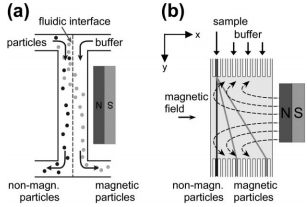
\includegraphics[width=0.8\linewidth]{images/sorting-force.png}\\
\hspace*{11pt}\hbox{\scriptsize \thinspace{\tiny\itshape Pamme, Lab Chip. 2007}}
% Pamme Lab Chip. 2007

% Zhao and Papautsky Lab Chip. 2013, 13, 1121
% Wang and Papautsky Lab Chip. 2015, 15, 1330
\end{figure}
\end{columns}
\end{frame}

\begin{frame}{Rapid Diffusion Enables Oxygen Control}
\begin{columns}[c] % The "c" option specifies centered vertical alignment while the "t" option is used for top vertical alignment
\column{.5\textwidth} % Left column and width
%\textbf{Heading}
\begin{figure}
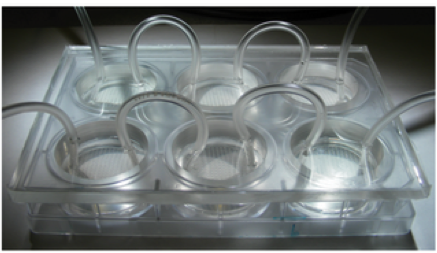
\includegraphics[width=.8\linewidth]{images/oppegard1.png}\\
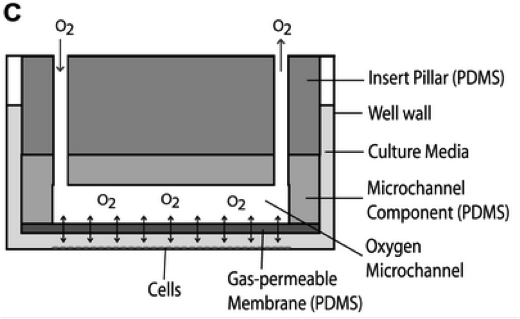
\includegraphics[width=.8\linewidth]{images/oppegard2.png}\\
\hspace*{11pt}\hbox{\scriptsize \thinspace{\tiny\itshape Oppegard et al. Plos One 2009}}
\end{figure}
\column{.5\textwidth} % Left column and width
\begin{figure}
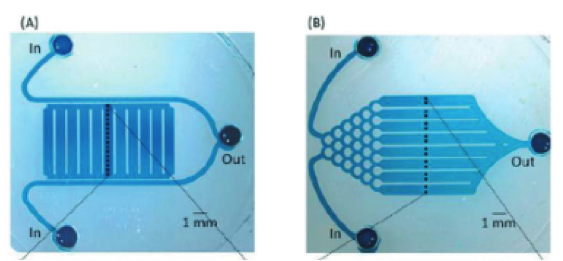
\includegraphics[width=0.7\linewidth]{images/lo1.png}\\
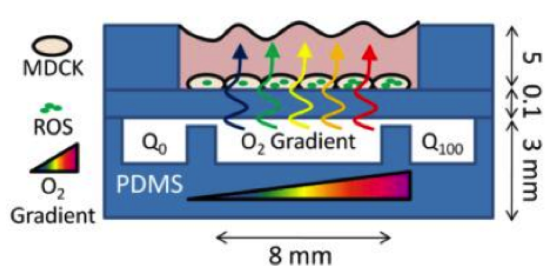
\includegraphics[width=0.7\linewidth]{images/lo2.png}\\
\hspace*{11pt}\hbox{\scriptsize \thinspace{\tiny\itshape Lo et al. Lab Chip, 2010 10(18): 2394–2401}}
\end{figure}
\end{columns}
\end{frame}

\begin{frame}{Droplet Microfluidics}
% droplets are formed from imiscable fluids
% many techniques have been developed to create droplets on chip.
% advantages include formation of monodisperse droplets, and ability to minipulate on chip
% generation techniques, T-junction, flow flocusing, sieve devices

%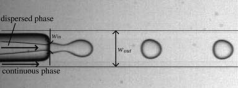
\includegraphics[width=0.6\linewidth]{images/co-axial.png}
%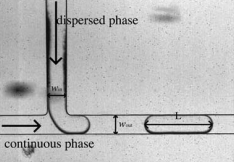
\includegraphics[width=0.6\linewidth]{images/t-junction.png}
%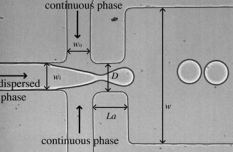
\includegraphics[width=0.6\linewidth]{images/flow-focusing.png}
% Baroud et al. Lab Chip, 2010, 10, 2032–2045.

% specific applications: 
%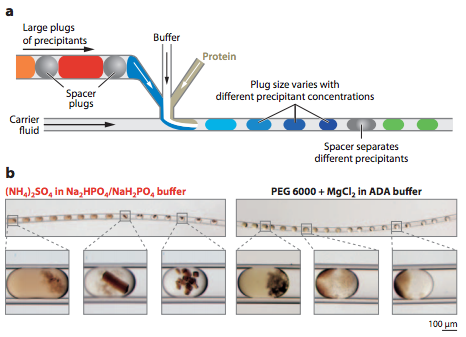
\includegraphics[width=0.6\linewidth]{images/crystallization.png}
%Li and Ismagilov, Annu. Rev. Biophys. 2010. 39:139–58
%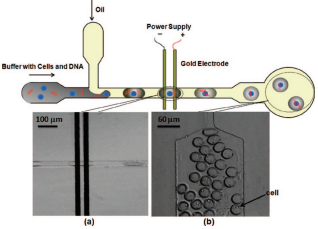
\includegraphics[width=0.6\linewidth]{images/poration.png}
% Zhan et al. Anal. Chem. 2009, 81, 2027–2031. Poration of Chinese Hamster Ovary (CHO) cells
\begin{figure}
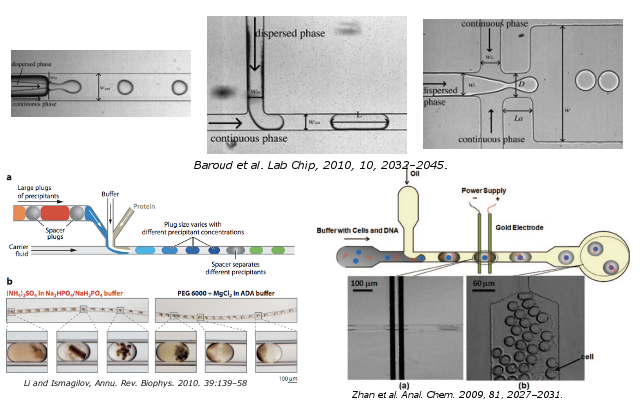
\includegraphics[width=1\linewidth]{images/droplets.png}
\end{figure}
\end{frame}

\begin{frame}{Droplet Microfluidics with cells}
%\textbf{Heading}
\animategraphics[loop,controls,width=.7\linewidth]{25}{images/drop/drop-}{0}{579}\\
\animategraphics[loop,controls,width=.7\linewidth]{25}{images/encap/encap-}{0}{499}\\
\hspace*{11pt}\hbox{\scriptsize \thinspace{\tiny\itshape Mazutis Nature Protocols 8, 870–891 (2013).}}
% Mazutis Nature Protocols 8, 870–891 (2013).
\end{frame}

\begin{frame}{Fabrication of Microfluidic devices - Soft-Photolithography}
\begin{figure}
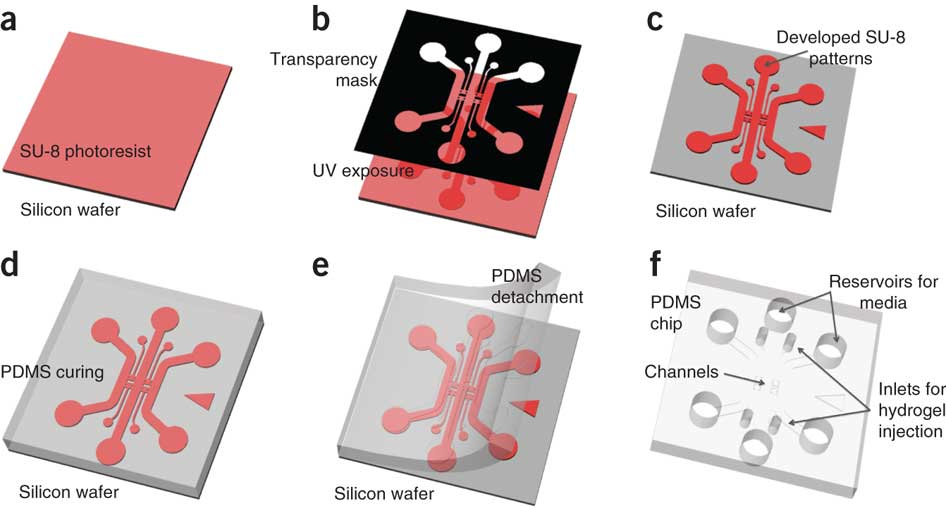
\includegraphics[width=0.8\linewidth]{images/soft-photolithography.jpg}\\
\hspace*{11pt}\hbox{\scriptsize \thinspace{\tiny\itshape Shin et al. Nature Protocols 7, 1247–1259 (2012).}}
\end{figure}
\end{frame}

\begin{frame}{3D-Printing - Additive Manufacturing }
\begin{figure}
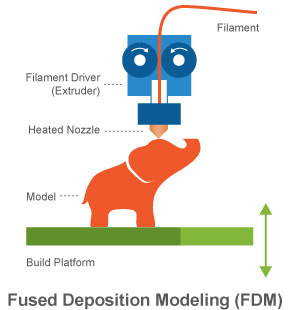
\includegraphics[width=0.25\linewidth]{images/fdm.jpg}
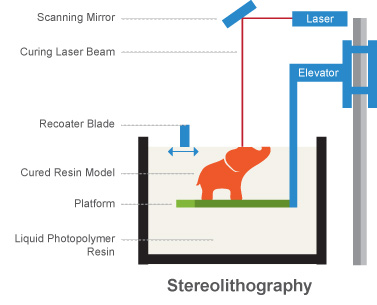
\includegraphics[width=0.3\linewidth]{images/stereolithography.jpg}
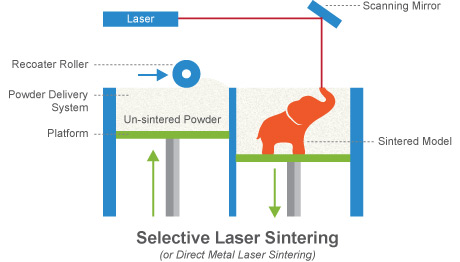
\includegraphics[width=0.37\linewidth]{images/selective-laser-sintering.jpg}\\
	\hspace*{11pt}\hbox{\scriptsize \thinspace{\tiny\itshape PrintSpace.com}}
\end{figure}
\end{frame}

\begin{frame}{3D-Printing as Alternative to Microfabrication}
\begin{columns}[c] % The "c" option specifies centered vertical alignment while the "t" option is used for top vertical alignment
\column{.66\textwidth} % Left column and width
%\textbf{Hypoxic Workstations}
\begin{figure}
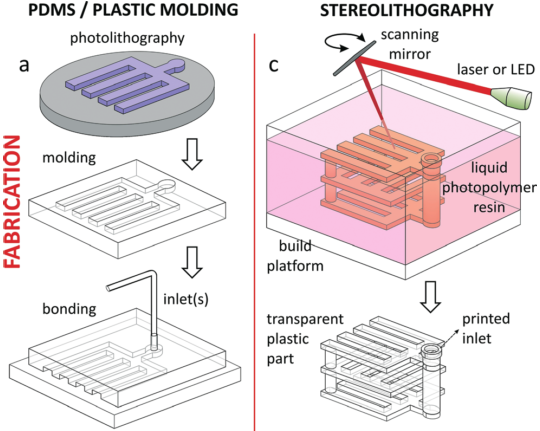
\includegraphics[width=0.8\linewidth]{images/3D-fab.png}\\
\hspace*{11pt}\hbox{\scriptsize \thinspace{\tiny\itshape Au et al. Lab Chip. 2014}}
 \end{figure}
\column{.33\textwidth} % Right column and width
%\textbf{Microfluidic Devices}
\begin{figure}
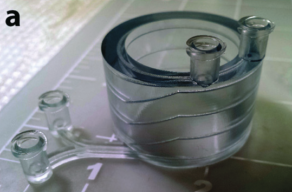
\includegraphics[width=1\linewidth]{images/folch1.png}\\
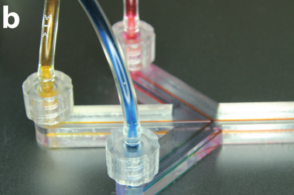
\includegraphics[width=1\linewidth]{images/folch2.png}\\
\hspace*{11pt}\hbox{\scriptsize \thinspace{\tiny\itshape Au et al. Lab Chip. 2014}}
 \end{figure}
\end{columns}
\end{frame}

%------------------------------------------------
\section{Specific Aim 1 : Demonstrate a microfluidic approach for co-encapsulation of two strains of strep to observe single gene transfer events}
%------------------------------------------------

\begin{frame}{Tango Device - Co-Encapsulation and Observation of Gene Transfer}
\begin{figure}
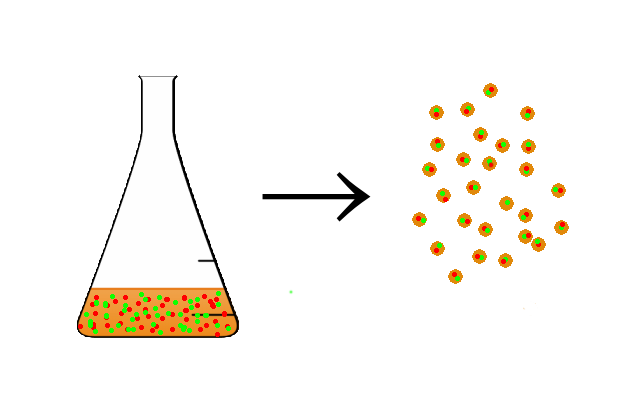
\includegraphics[width=0.8\linewidth]{images/flask-droplets.png}
\end{figure}
\end{frame}

\begin{frame}{Horizontal Gene Transfer}
\begin{figure}
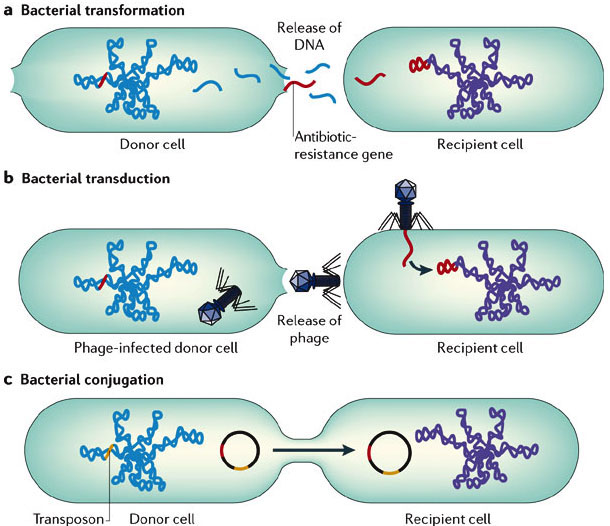
\includegraphics[width=0.65\linewidth]{images/HGT.jpg}\\
\hspace*{11pt}\hbox{\scriptsize \thinspace{\tiny\itshape Furuya and Lowy. Nature Reviews Microbiology 4, 36-45, 2006}}
%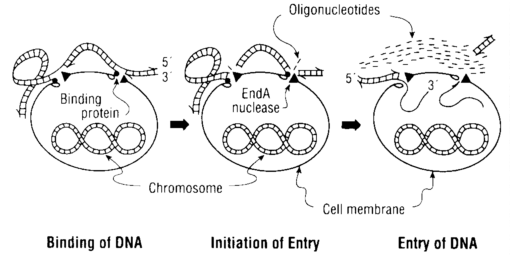
\includegraphics[width=0.8\linewidth]{images/intake.png}
\end{figure}
\end{frame}

\begin{frame}{Uptake of Free DNA by a Competent Cell}
\begin{figure}
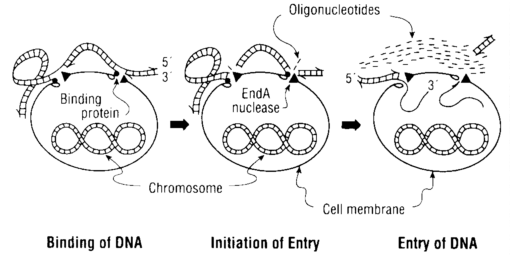
\includegraphics[width=0.5\linewidth]{images/intake.png}\\
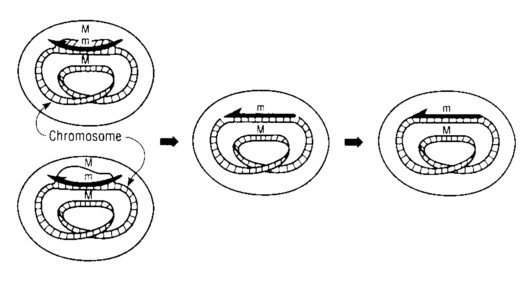
\includegraphics[width=0.5\linewidth]{images/recombination.png}\\
\hspace*{11pt}\hbox{\scriptsize \thinspace{\tiny\itshape Lacks. MICROBIAL DRUG RESISTANCE Volume 3, Number 4, 1997.}}
% Lacks. MICROBIAL DRUG RESISTANCE Volume 3, Number 4, 1997.
\end{figure}
\end{frame}

\begin{frame}{Impact of \textit{S. pneumoniae}}
\begin{figure}
\begin{itemize}
\item 14.5 million cases of serious disease, 826,000 deaths, in children less than 5 years
\item pneumonia, meningitis and sepsis
%  O’Brien et al. Lancet 2009, Vol 374.
\end{itemize}
\end{figure}
\begin{figure}
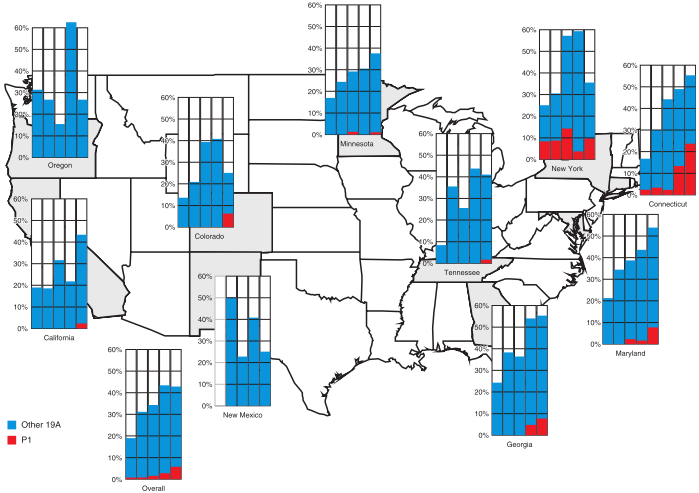
\includegraphics[width=0.6\linewidth]{images/spread-of-p1.png}\\
\hspace*{11pt}\hbox{\scriptsize \thinspace{\tiny\itshape Golubchik. Nature Genetics. March 2012, Vol 44, Num 3.}}
%Golubchik. Nature Genetics. March 2012, Vol 44, Num 3.
%Spread of P1 vaccine escape recombinat 2003-2007
\end{figure}
\end{frame}

\begin{frame}{In vivo}
\begin{figure}

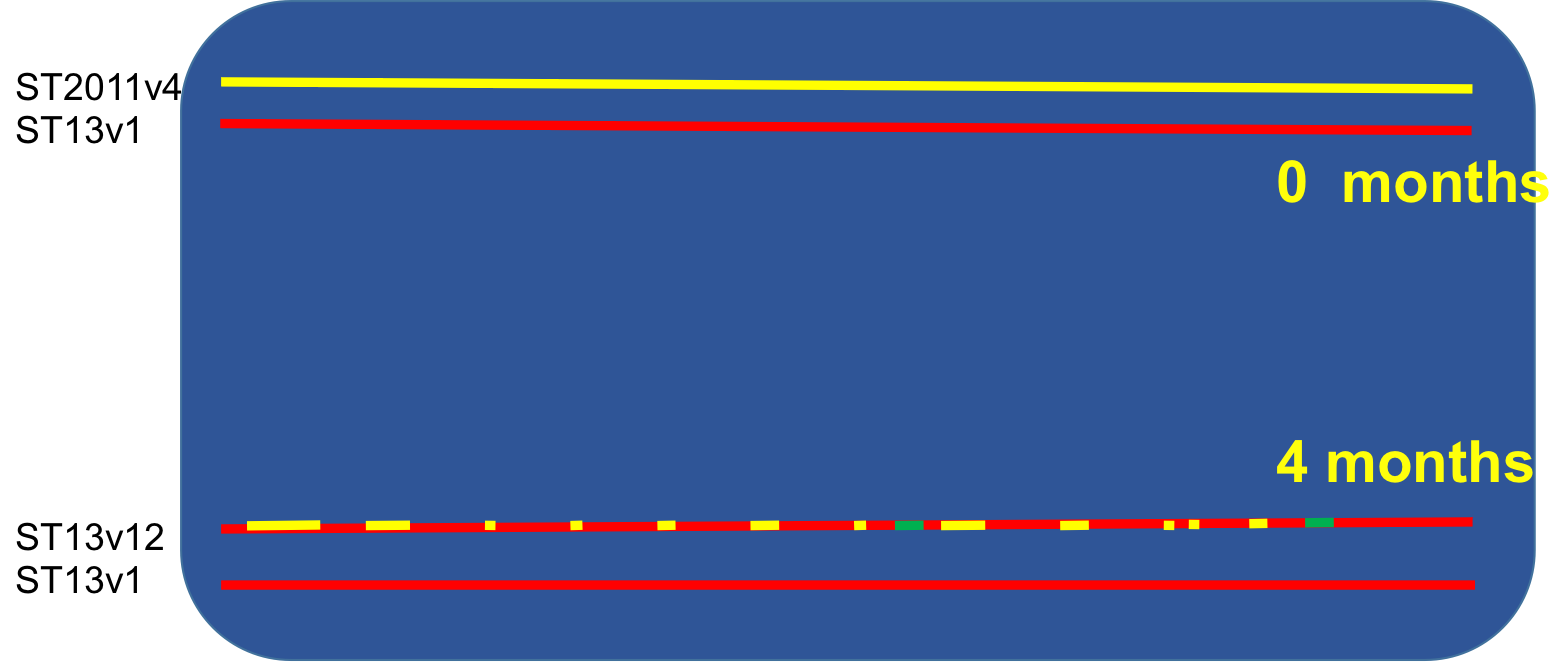
\includegraphics[width=0.5\linewidth]{images/transfer-vivo.png}\\
\hspace*{11pt}\hbox{\scriptsize \thinspace{\tiny\itshape Hiller 2010 (Reproduced by Morrison) }}\\
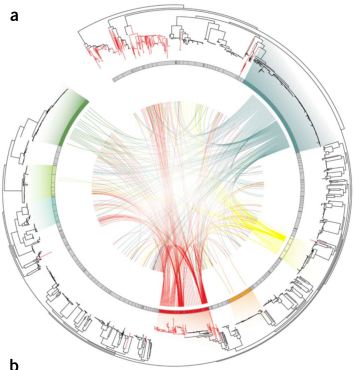
\includegraphics[width=0.3\linewidth]{images/phylogentic-crosses.png}\\
\hspace*{11pt}\hbox{\scriptsize \thinspace{\tiny\itshape Chewapreecha. Nature Genetics. 2014, Vol 46, Num 3.}}
% Chewapreecha. NATURE GENETICS VOLUME 46 | NUMBER 3 | MARCH 2014

% Hiller et al. Plos Pathogens September 2010 | Volume 6 | Issue 9 | e1001108
%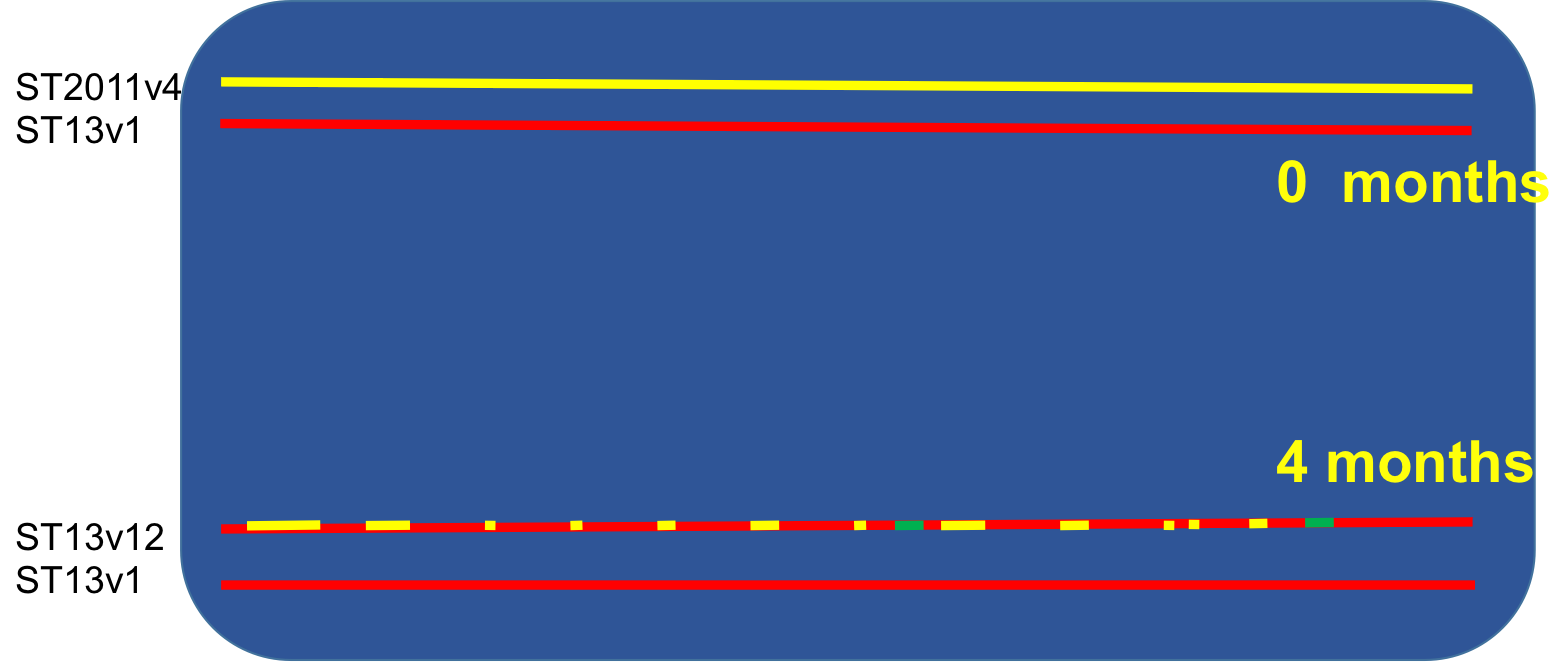
\includegraphics[width=0.8\linewidth]{images/transfer-vivo.png}
\end{figure}
\end{frame}

\begin{frame}{Competence is induced and involves attack on donor cell}
\begin{columns}[c] % The "c" option specifies centered vertical alignment while the "t" option is used for top vertical alignment
\column{.5\textwidth}
\begin{figure}
\begin{itemize}
\item Competence is CSP concentration dependent, 1-10 ng, $10^{7}$ cells/mL
\item Fraction of cells lyse at critical CSP concentration
\item Competence-induced cells lyse competence-deficient cells 
\item Lysis is dependent on activity of CbpD protein
%\item Transformation studied in populations in suspension
%\item Extent of resulting recombination is not as much as observed in vivo
%\item Single transfer events are unknown
% nearly 90 years ago Griffith first discovered genetic transformation. A nonvirulent strain was observed to gain virulence from a heat killed virulent strain.
% 1928 Study non virulent strain is cultured in media with heat killed virulent strain. At certian time point virulence emerges in live strain
% Kausmally et al. CSP is a peptide pheremone 
\end{itemize}
\end{figure}
%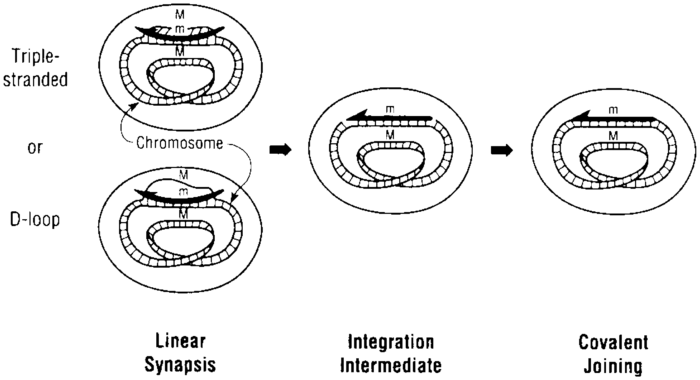
\includegraphics[width=0.8\linewidth]{images/transformation}
\column{.5\textwidth} 
\begin{figure}
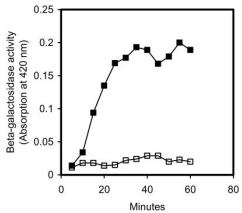
\includegraphics[width=0.6\linewidth]{images/beta-g-vs-time.png}\\
\hspace*{11pt}\hbox{\scriptsize \thinspace{\tiny\itshape Steinmoen et al. PNAS 2002, Vol. 99, no. 11, 7681-7686}}\\
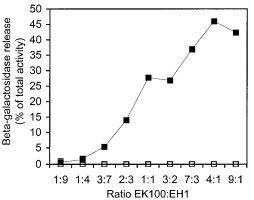
\includegraphics[width=0.6\linewidth]{images/beta-g-ratio.png}\\
\hspace*{11pt}\hbox{\scriptsize \thinspace{\tiny\itshape Steinmoen et al. J. Bacteriology, Dec. 2003, p. 7176–7183}}
%Steinmoen et al. PNAS 2002, Vol. 99, no. 11, 7681-7686
% Steinmoen et al. J. Bacteriology, Dec. 2003, p. 7176–7183
\end{figure}
\end{columns}
\end{frame}

\begin{frame}{Aim: Co-encapsulation of two strains of \textit{S. pneumoniae} to observe single gene transfer events}
\begin{itemize}
%\item Transformation studied in populations in suspension
%\item Extent of resulting recombination is not as much as observed in vivo
%\item Single transfer events are unknown
\item Isolate two cells in a confined area to determine what happens in a single gene transfer
\item Attack strain with inducible competence (Does not produce CSP), RFP labeled
\item Non-competent victim strain (cannot sense CSP), GFP expressing
\item Encapsulate attacker-victim pairs in Droplets
\end{itemize}
\begin{figure}
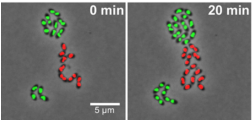
\includegraphics[width=0.5\linewidth]{images/red-green.png}\\
\hspace*{11pt}\hbox{\scriptsize \thinspace{\tiny\itshape Kjos et al. Journal of Bacteriology 2015 Vol 197 No 5.}}
%Kjos et al. Journal of Bacteriology 2015 Vol 197 No 5.
\end{figure}
\end{frame}

\begin{frame}{Inspiration - Algae Encapsulation Device}
\begin{figure}
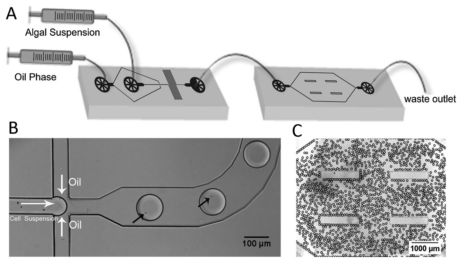
\includegraphics[width=.9\linewidth]{images/algae-droplets.png}\\
\hspace*{11pt}\hbox{\scriptsize \thinspace{\tiny\itshape Pan et al. Integr. Biol., 2011, 3, 1043–1051}}
\end{figure}
\end{frame}

\begin{frame}{Device Design}
\begin{columns}[c] % The "c" option specifies centered vertical alignment while the "t" option is used for top vertical alignment
\column{.7\textwidth} % Left column and width
\begin{figure}
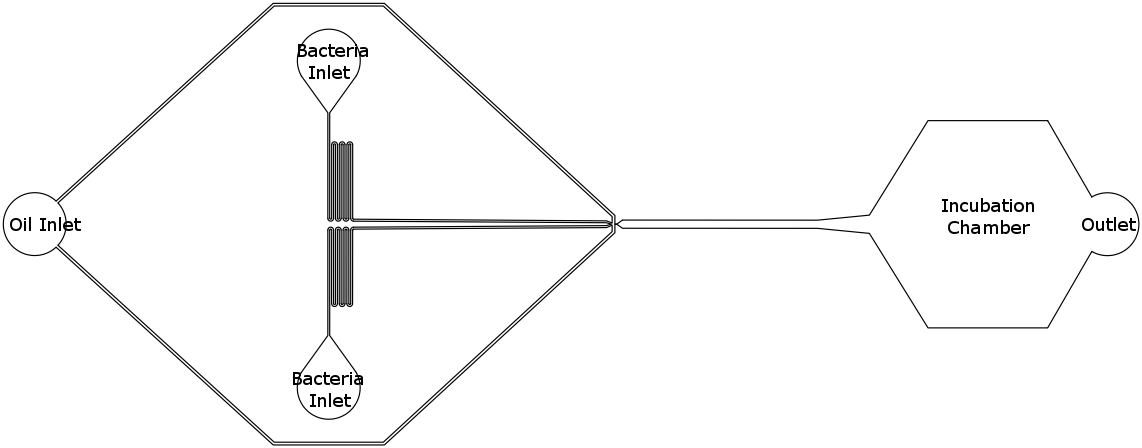
\includegraphics[width=1\linewidth]{images/chip-design.png}
\end{figure}
\column{.3\textwidth} 
\begin{figure}
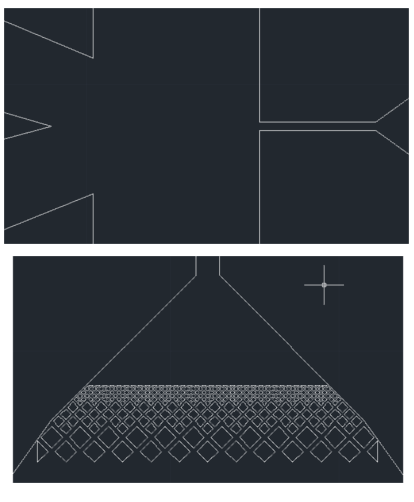
\includegraphics[width=1\linewidth]{images/neck-and-filters.png}
\end{figure}
\end{columns}
\end{frame}

\begin{frame}{Droplet Generation}
\begin{columns}[c] % The "c" option specifies centered vertical alignment while the "t" option is used for top vertical alignment
\column{.45\textwidth} % Left column and width
%\textbf{Heading}
\begin{itemize}
\item Oil flowrate of 150 $\mu$mL/h, aqueous 50 $\mu$mL/h 
\item Neck width of 5 $\mu$m
\item Droplets of 5-10 $\mu$m are generated
\item 5 femtoliter droplets 
\end{itemize}
\column{.5\textwidth} % Right column and width
 \animategraphics[loop,controls,width=.7\linewidth]{5}{images/generator-seq/generator-}{63}{89}
\end{columns}
\end{frame}

\begin{frame}{Beads in Droplets}
\begin{columns}[c] % The "c" option specifies centered vertical alignment while the "t" option is used for top vertical alignment
\column{.45\textwidth} % Left column and width
%\textbf{Heading}
\begin{itemize}
\item Green and red florescent beads of 1 $\mu$m diameter
\item 4x$10^{9}$ beads/ml
\item 20\% occupancy, 5\% R\&G 
% timelapse 
\end{itemize}
\column{.5\textwidth} % Right column and width
 \animategraphics[loop,controls,width=.6\linewidth]{5}{images/beads-seq/beads-}{0}{35}
\end{columns}
\end{frame}

\begin{frame}{Full Experiment Procedure}
\begin{figure}
\begin{enumerate}
\item Encapsulate attacker and victim strains in droplets
\item Incubate droplets in the device and observe attack
\item Break the emulsion, dilute and plate
\item Assess gene transfer with whole genome sequencing of remaining cultures
\end{enumerate}
\end{figure}
\end{frame}

\begin{frame}{Expected Results}
\begin{figure}
\begin{itemize}
\item Encapsulate cells and determine occupancy
\item Image cells during incubation to observe attack
\item Ultimately determine what can be expected from a single transfer event
\end{itemize}
\end{figure}
\begin{figure}
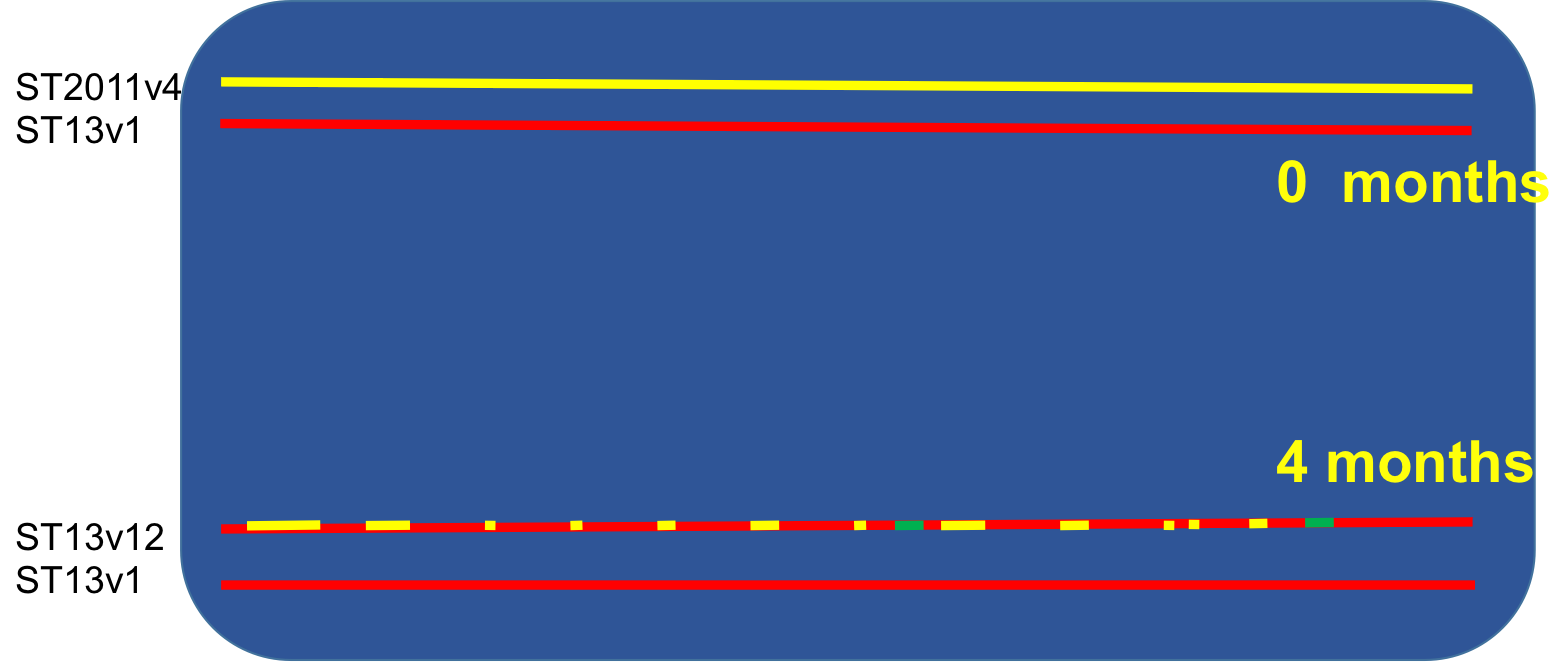
\includegraphics[width=0.8\linewidth]{images/transfer-vivo.png}\\
\hspace*{11pt}\hbox{\scriptsize \thinspace{\tiny\itshape Hiller 2010 (Reproduced by Morrison) }}
\end{figure}
\end{frame}

\begin{frame}{Potential Difficulties}
\begin{figure}
\begin{itemize}
\item Cells may not become competent due to encapsulation
\item Cells may not physically meet
\item Attack or transformation may require more than 2 cells
\item Confinement may cause lysis of both cells
 \end{itemize}
\end{figure}
\end{frame}

%\begin{frame}{Index of refraction Mis-match}
%\begin{figure}
%
\includegraphics[width=0.8\linewidth]{images/lenses.png}
%\end{figure}
%\end{frame}

%------------------------------------------------
\section{Specific Aim 2: Develop an easy to use and fabricate oxygen control insert for a 24-well plate}
%------------------------------------------------

\begin{frame}{3D-Printed Oxygen Control Insert}
\begin{figure}
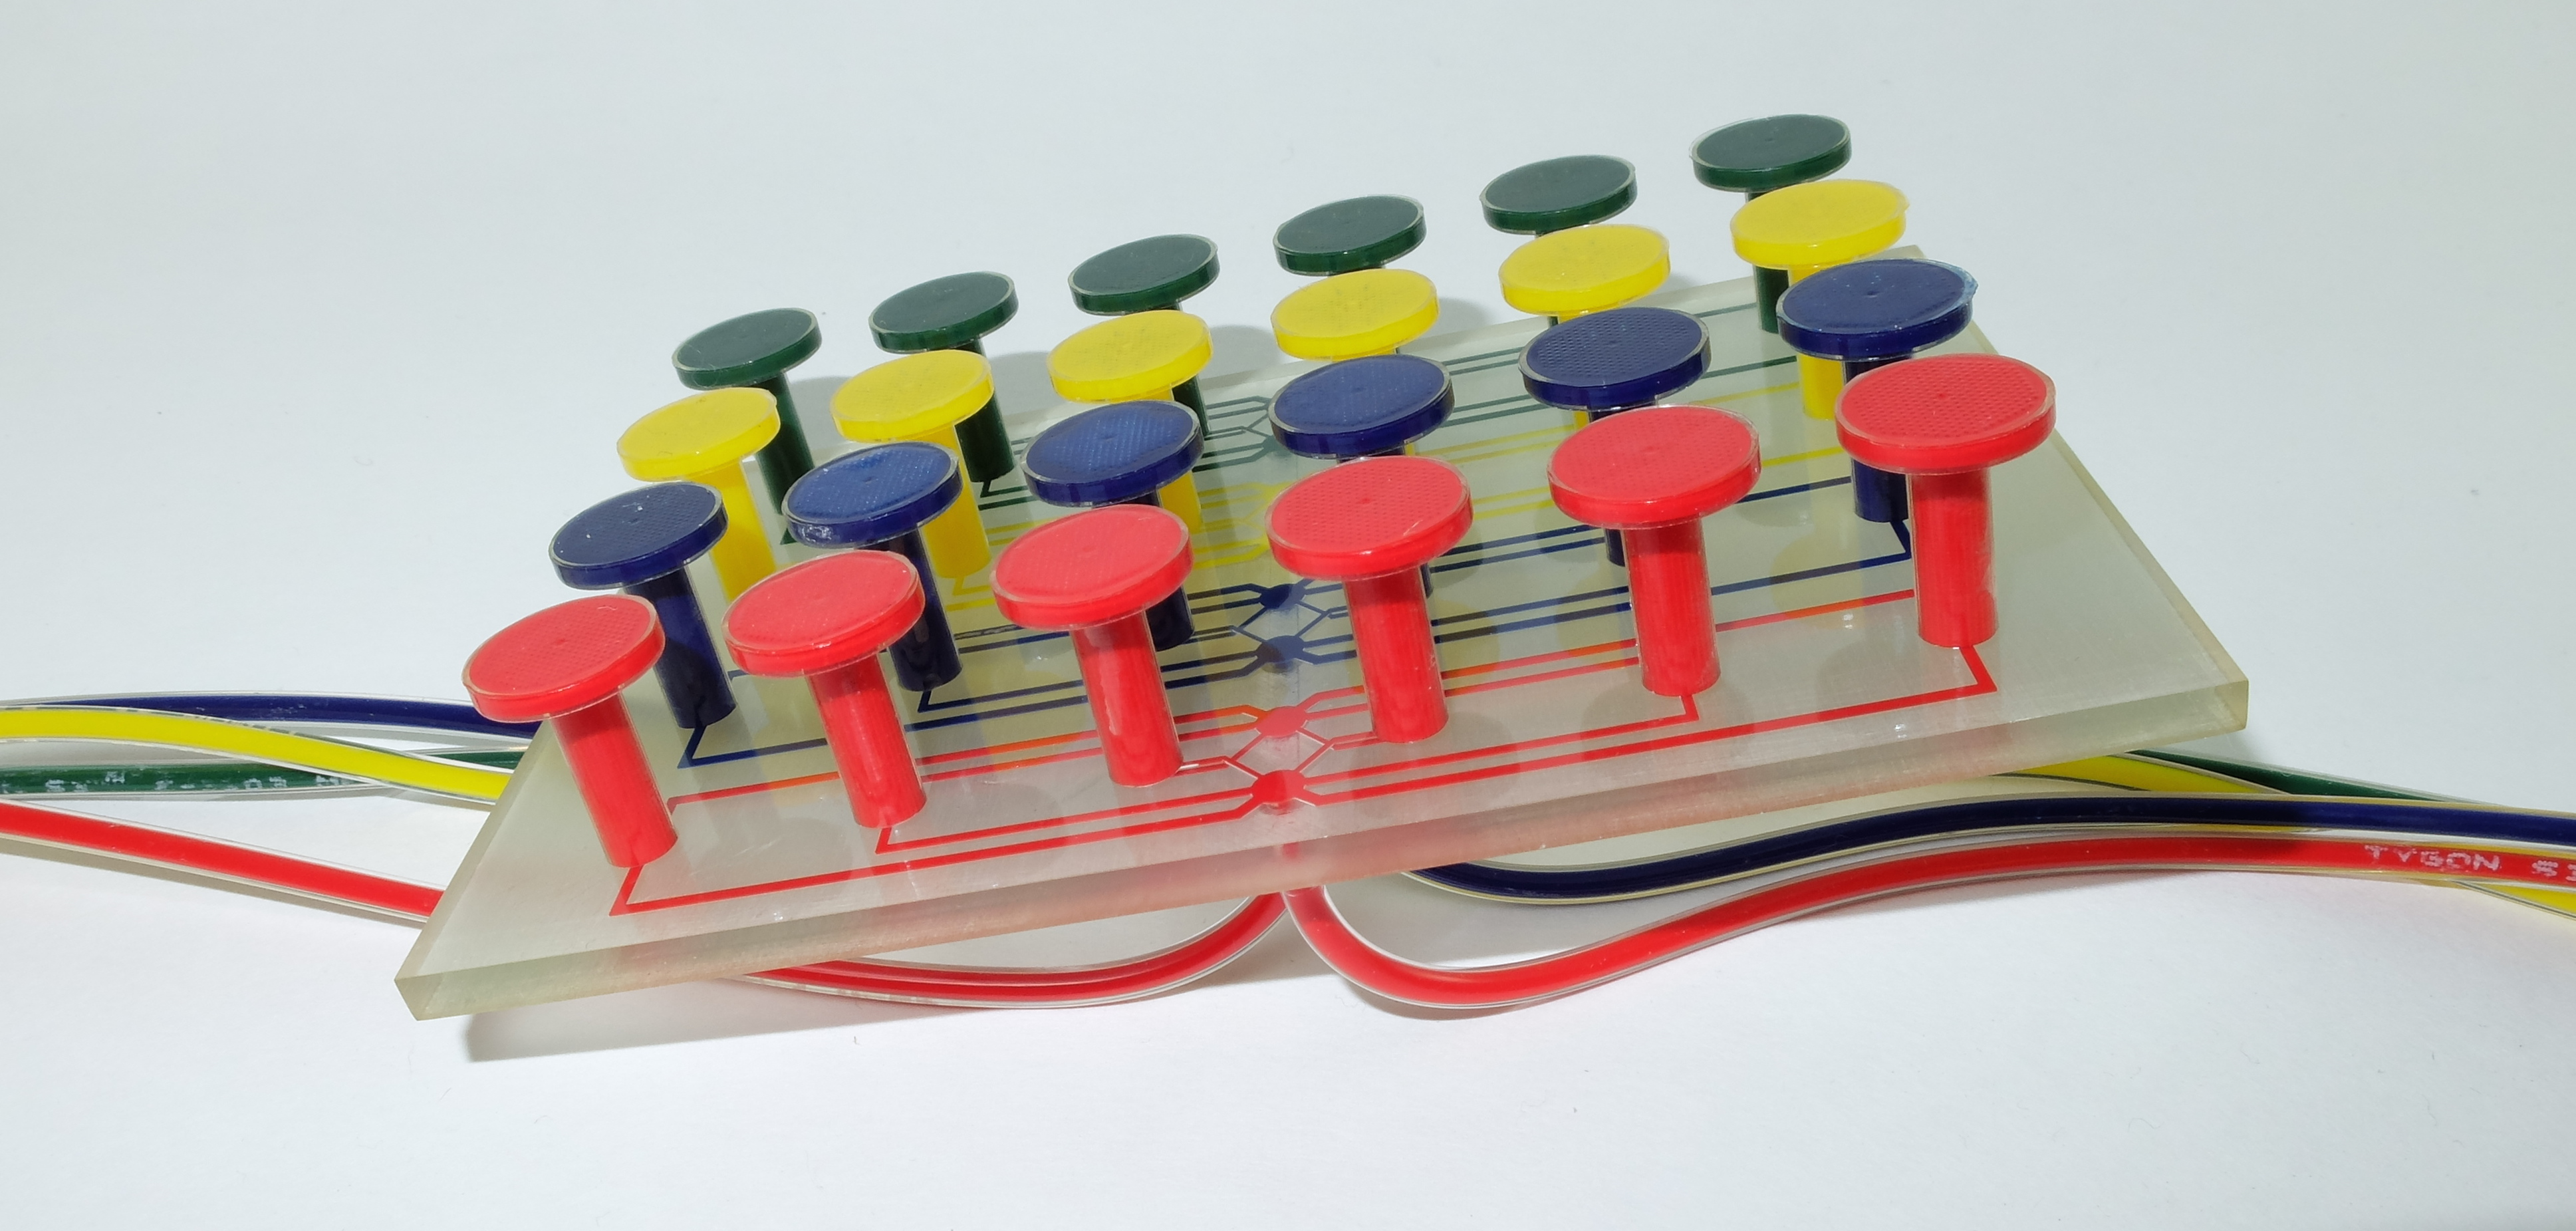
\includegraphics[width=0.9\linewidth]{images/insert.JPG}
\end{figure}
\end{frame}

\begin{frame}{Oxygen in Vivo Versus Oxygen in Research}
\begin{columns}[c] % The "c" option specifies centered vertical alignment while the "t" option is used for top vertical alignment
\column{.35\textwidth} % Left column and width
%\textbf{Heading}
\begin{itemize}
\item Typically ignored, culture studied at 21\%
\item Equipment is inconvenient for oxygenating to multiple levels and is expensive
\item Microfluidic oxygen devices must be expertly made and operated
% timelapse 
\end{itemize}
\column{.65\textwidth} % Right column and width
\begin{figure}
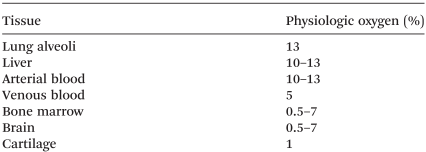
\includegraphics[width=1\linewidth]{images/oxygen-table.png}\\
\hspace*{11pt}\hbox{\scriptsize \thinspace{\tiny\itshape Brennan et al. Lab Chip, 2014, 14, 4305–4318 }}
 \end{figure}
\end{columns}
\end{frame}

\begin{frame}{Methods for Oxygen Control}
\begin{columns}[c] % The "c" option specifies centered vertical alignment while the "t" option is used for top vertical alignment
\column{.5\textwidth} % Left column and width
\textbf{Hypoxic Workstations}
\begin{figure}
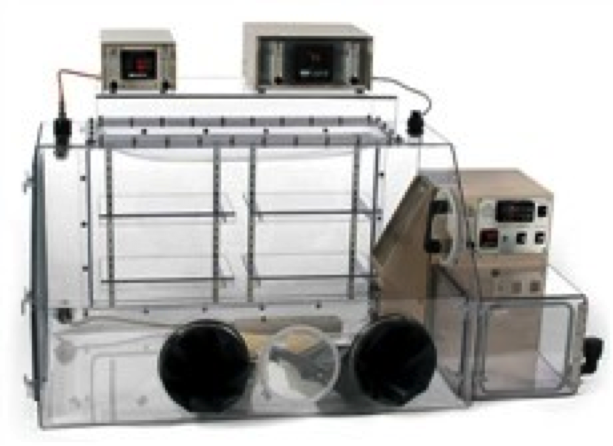
\includegraphics[width=0.8\linewidth]{images/hypoxia-workstation.png}
 \end{figure}
\column{.5\textwidth} % Right column and width
\textbf{Microfluidic Devices}
\begin{figure}
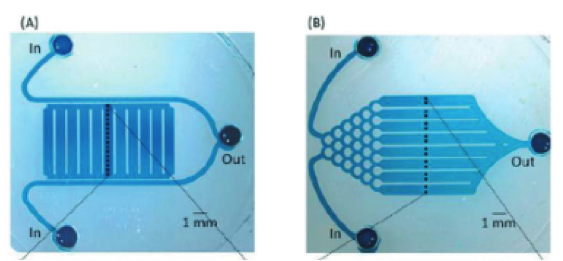
\includegraphics[width=0.7\linewidth]{images/lo1.png}\\
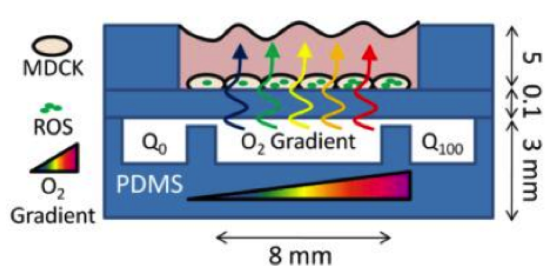
\includegraphics[width=0.7\linewidth]{images/lo2.png}\\
\hspace*{11pt}\hbox{\scriptsize \thinspace{\tiny\itshape Lo et al. Lab Chip, 2010 10(18): 2394–2401}}
 \end{figure}
\end{columns}
\end{frame}

\begin{frame}{Aim: Develop an easy to use and fabricate oxygen control system for researchers}
\begin{columns}[c] % The "c" option specifies centered vertical alignment while the "t" option is used for top vertical alignment
\column{.5\textwidth} % Left column and width
\begin{itemize}
\item Use Multi-well plate platform
\item 3D-printing - outsource fabrication
\item Integrate functionality 
 \end{itemize}
\column{.5\textwidth} % Right column and width
%\textbf{Microfluidic Devices}
\begin{figure}
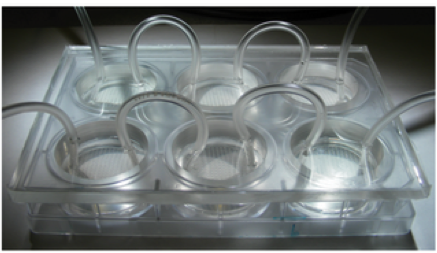
\includegraphics[width=.8\linewidth]{images/oppegard1.png}\\
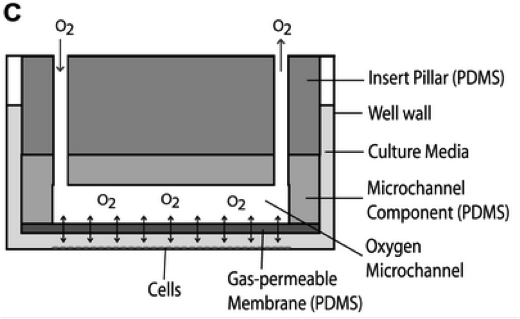
\includegraphics[width=.8\linewidth]{images/oppegard2.png}\\
\hspace*{11pt}\hbox{\scriptsize \thinspace{\tiny\itshape Oppegard et al. Plos One 2009}}
 \end{figure}
\end{columns}
\end{frame}

\begin{frame}{3D-Printing}
\begin{columns}[c] % The "c" option specifies centered vertical alignment while the "t" option is used for top vertical alignment
\column{.66\textwidth} % Left column and width
%\textbf{Hypoxic Workstations}
\begin{figure}
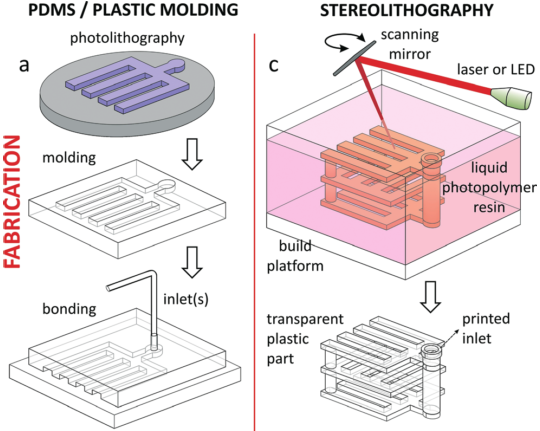
\includegraphics[width=0.8\linewidth]{images/3D-fab.png}\\
\hspace*{11pt}\hbox{\scriptsize \thinspace{\tiny\itshape Au et al. Lab Chip. 2014}}
 \end{figure}
\column{.33\textwidth} % Right column and width
%\textbf{Microfluidic Devices}
\begin{figure}
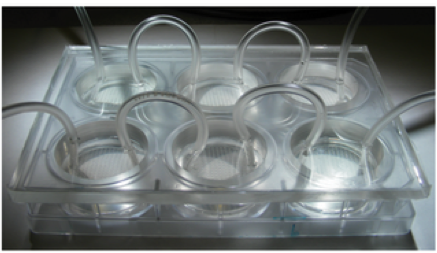
\includegraphics[width=1\linewidth]{images/oppegard1.png}\\
\hspace*{11pt}\hbox{\scriptsize \thinspace{\tiny\itshape Oppegard et al. Plos One 2009}}
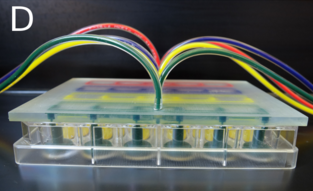
\includegraphics[width=1\linewidth]{images/insert-plate.png}

 \end{figure}
\end{columns}
\end{frame}

\begin{frame}{Insert Design}
\begin{figure}
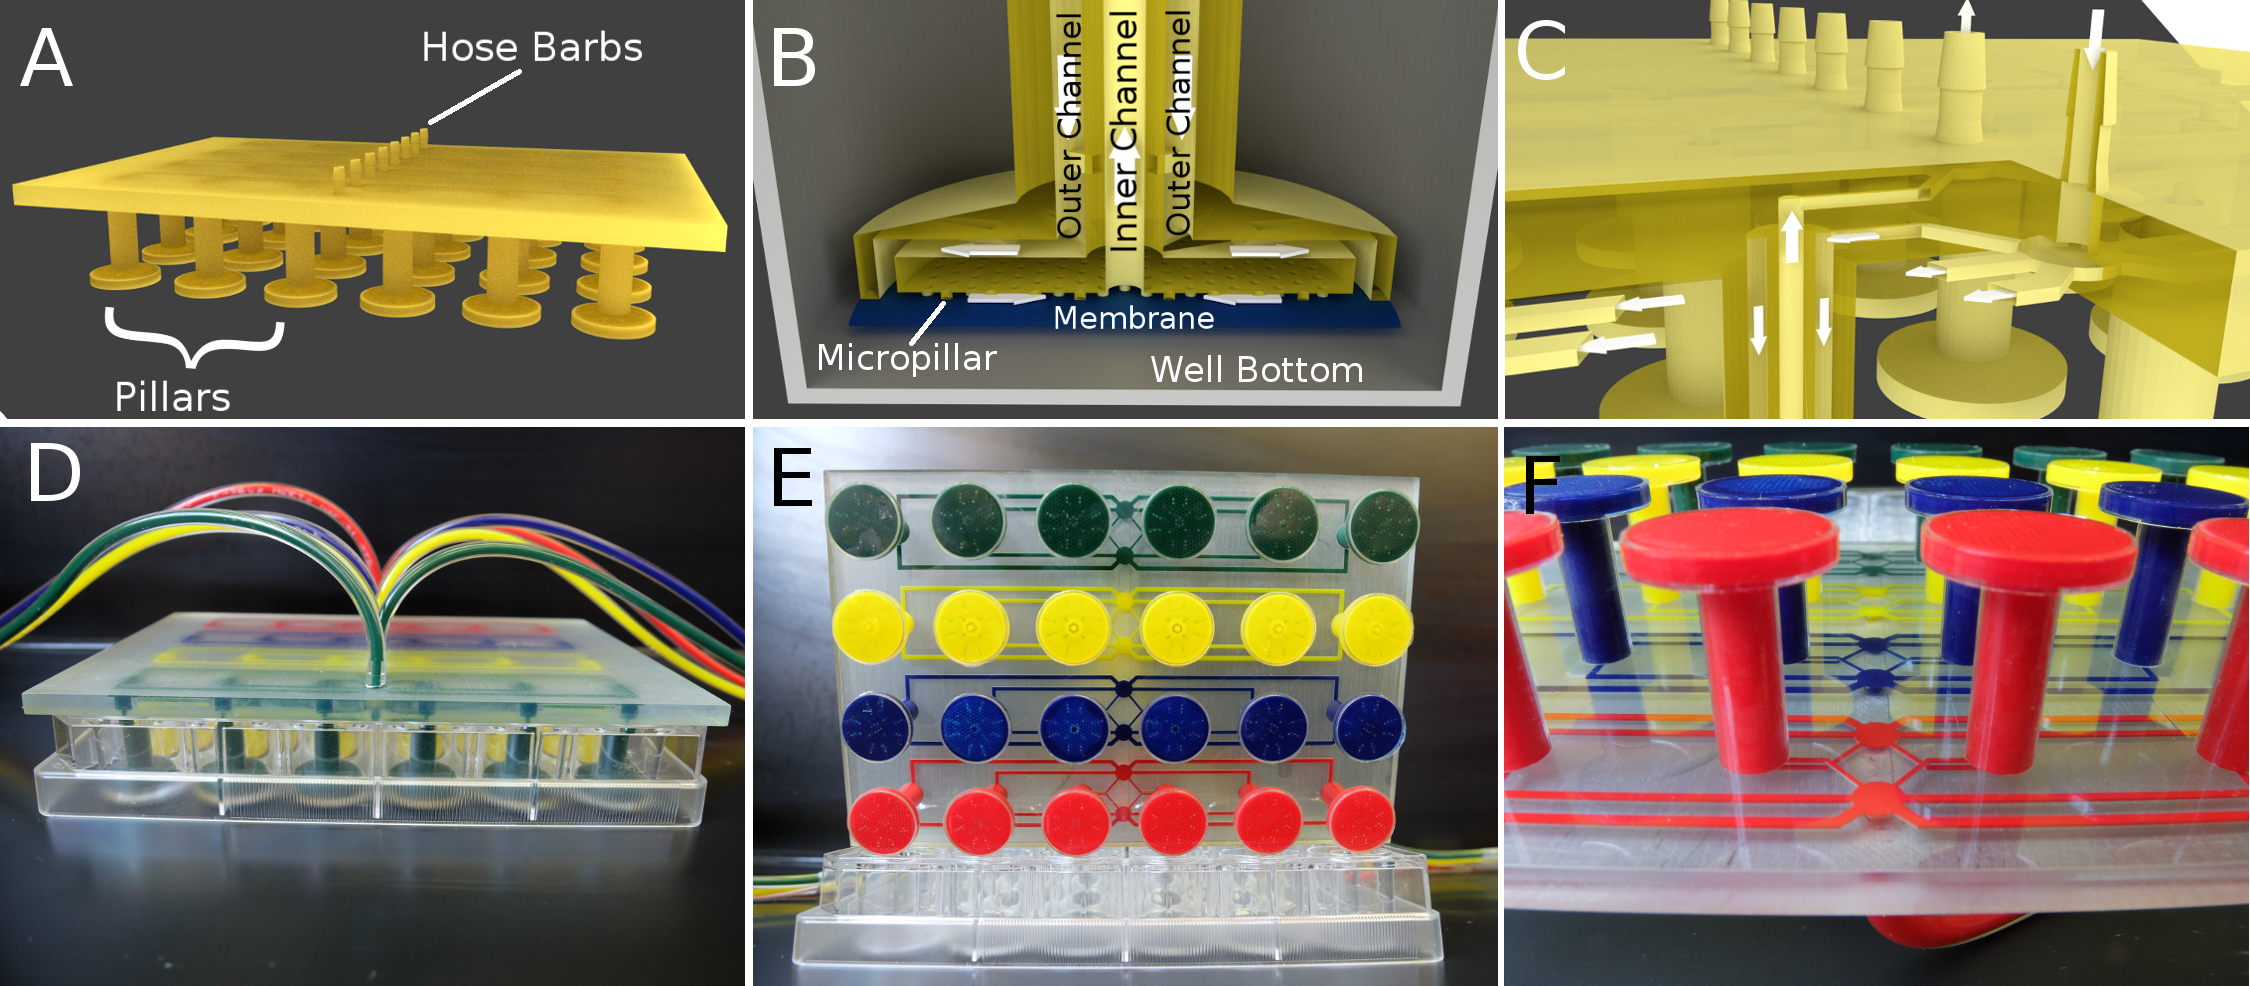
\includegraphics[width=1\linewidth]{images/insert.png}\\
\hspace*{11pt}\hbox{\scriptsize \thinspace{\tiny\itshape Brennan et al. Plos One 2015}}
 \end{figure}
\end{frame}

\begin{frame}{Oxygen Performance - Stern Volmer Analysis}
\begin{columns}
\column{.5\textwidth} % Left column and width
\begin{figure}
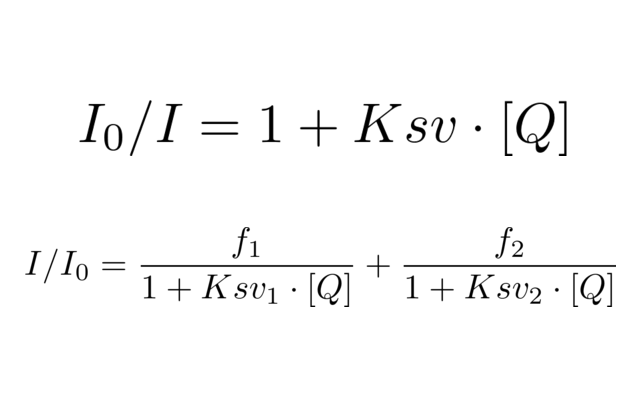
\includegraphics[width=.6\linewidth]{images/stern-volmer-equ.png}\\
\includegraphics[width=1\linewidth]{images/oxygen-time.png}
\end{figure}
\column{.5\textwidth} % Right column and width
%\textbf{Microfluidic Devices}
\begin{figure}
\includegraphics[width=.8\linewidth]{images/stern-volmer-plots.png}
 \end{figure}
\end{columns}
\end{frame}

\begin{frame}{Bioverification}
\begin{figure}
\includegraphics[width=0.8\linewidth]{images/hypoxia-pcr.png}\\
\hspace*{11pt}\hbox{\scriptsize \thinspace{\tiny\itshape Brennan et al. Plos One 2015}}
 \end{figure}
\end{frame}
% Vegf regulation due to hypoxia

\begin{frame}{Expanding and improving the device}
\begin{columns}
\column{.4\textwidth} % Left column and width
\begin{itemize}
\item Membrane material
\item Media exchange
\item Pattering of oxygen in wells 
 \end{itemize}
\column{.6\textwidth} % Right column and width
%\textbf{Microfluidic Devices}
\begin{figure}
\includegraphics[width=.8\linewidth]{images/oppegard3.png}\\
\hspace*{11pt}\hbox{\scriptsize \thinspace{\tiny\itshape Oppegard et al. Plos One 2009}}

 \end{figure}
\end{columns}
\end{frame}

\begin{frame}{GitHub}
\begin{figure}
\includegraphics[width=0.8\linewidth]{images/github-insert.png}
\end{figure}
\end{frame}

%------------------------------------------------
\section{Specific Aim 3: Develop a 3D printable micropipette and compare its performance to commercial versions}
%------------------------------------------------

\begin{frame}{Open Design Scientific Tools}
\begin{columns}
\column{.5\textwidth} % Left column and width
\begin{figure}
\includegraphics[width=1\linewidth]{images/opensource-software.jpeg}
 \end{figure}
\column{.5\textwidth} % Right column and width
%\textbf{Microfluidic Devices}
\begin{figure}
\includegraphics[width=1\linewidth]{images/opensource-hardware.png}
 \end{figure}
\end{columns}
\end{frame}

\begin{frame}{3D-Printed Scientific Tools}
\begin{figure}
	\includegraphics[width=.8\linewidth]{images/3D-printed-tools.png}\\
	%thing:1483 dremelfuge
	%thing:thing:26553 filterwheel
	%thing:77450 microscope
	\hspace*{11pt}\hbox{\scriptsize \thinspace{\tiny\itshape Thing:1483 Dremelfuge, Thing:26553 Filterwheel, Thing:77450 Microscope}}\\
	\hspace*{11pt}\hbox{\scriptsize \thinspace{\tiny\itshape Wijnen et al. 2014, Volume 9, Issue 9, e107216.}}
\end{figure}
\end{frame}

\begin{frame}{3D-Printed Pipettes}
	\begin{figure}
		\includegraphics[width=1\linewidth]{images/competitor-pipette.png}\\
		\hspace*{11pt}\hbox{\scriptsize \thinspace{\tiny\itshape Thing:159052 Laboratory pipette, Thing:25519 Briopipette}}
	\end{figure}
\end{frame}

\begin{frame}{Aim: Develop a 3D printable micropipette and compare to commercial versions}
\begin{itemize}
\item Use a consumer grade printer
\item Simple hardware
\item Adjustable to desired volume a priori
\item Comparable accuracy to a commercial pipette
 \end{itemize}
\end{frame}

\begin{frame}{Design of Pipette}
\begin{figure}
\includegraphics[width=0.8\linewidth]{images/pipette.png}
 \end{figure}
\end{frame}

\begin{frame}{Current Prototype}
\begin{itemize}
		\item Makerbot printable, \$5 USD including parts
		\item Uses syringe graduations to set volume
		\item Competitive with commercial pipettes in accuracy 
	\end{itemize}
\begin{figure}
\includegraphics[width=0.8\linewidth]{images/pipette-photo.png}
 \end{figure}
\end{frame}

\begin{frame}{Operating Procedure}
\animategraphics[loop,controls,width=1\linewidth]{1}{images/operation/operation-}{0}{3}
\begin{itemize}
\item Compare displacement from bottom and top stop with graduations
\item Adjust top stop with screw
\item Re-check displacement
\item Pipette
 \end{itemize}
\end{frame}

\begin{frame}{Preliminary Results}
\begin{figure}
		\includegraphics[width=.8\linewidth]{images/pipette-data.png}
		%\caption{Thingiverse things: 159052 and 255519}
	\end{figure}
\end{frame}

\begin{frame}{Future Approach}
\begin{itemize}
\item Add features such as ejector for tips
\item Push-push operation
\item improve user friendliness
\begin{figure}
		\includegraphics[width=.8\linewidth]{images/finnpipette.jpg}
	\end{figure}
 \end{itemize}
\end{frame}


\section{Conclusion and Thanks}

\begin{frame}{Wrap-Up}
\begin{figure}
	\includegraphics[width=1\linewidth]{images/wrap-up.png}
\end{figure}
\end{frame}

\begin{frame}{Acknowledgments}
	\textbf{Thank You}
	\begin{itemize}
		\item Dr. Morrison - Gene Transfer on a Chip
		\item Megan - Bioverification PCR
		\item Fahad - CAD 
		\item Dr. Eddington - Advisor 
		\item Committee 
	\end{itemize}
\end{frame}

\begin{frame}
\Huge{\centerline{Thank You}}
\end{frame}

%\subsection{Subsection Example} % A subsection can be created just before a set of slides with a common theme to further break down your presentation into chunks



%------------------------------------------------



%------------------------------------------------

%\begin{frame}
%\frametitle{Blocks of Highlighted Text}
%\begin{block}{Block 1}
%Lorem ipsum dolor sit amet, consectetur adipiscing elit. Integer lectus nisl, ultricies in feugiat rutrum, porttitor sit amet augue. Aliquam ut tortor mauris. Sed volutpat ante purus, quis accumsan dolor.
%\end{block}

%\begin{block}{Block 2}
%Pellentesque sed tellus purus. Class aptent taciti sociosqu ad litora torquent per conubia nostra, per inceptos himenaeos. Vestibulum quis magna at risus dictum tempor eu vitae velit.
%\end{block}

%\begin{block}{Block 3}
%Suspendisse tincidunt sagittis gravida. Curabitur condimentum, enim sed venenatis rutrum, ipsum neque consectetur orci, sed blandit justo nisi ac lacus.
%\end{block}
%\end{frame}

%------------------------------------------------

%\begin{frame}
%\frametitle{Multiple Columns}
%\begin{columns}[c] % The "c" option specifies centered vertical alignment while the "t" option is used for top vertical alignment

%\column{.45\textwidth} % Left column and width
%\textbf{Heading}
%\begin{enumerate}
%\item Statement
%\item Explanation
%\item Example
%\end{enumerate}

%\column{.5\textwidth} % Right column and width
%Lorem ipsum dolor sit amet, consectetur adipiscing elit. Integer lectus nisl, ultricies in feugiat rutrum, porttitor sit amet augue. Aliquam ut tortor mauris. Sed volutpat ante purus, quis accumsan dolor.

%\end{columns}
%\end{frame}

%------------------------------------------------
%\section{Second Section}
%------------------------------------------------

%\begin{frame}
%\frametitle{Table}
%\begin{table}
%\begin{tabular}{l l l}
%\toprule
%\textbf{Treatments} & \textbf{Response 1} & \textbf{Response 2}\\
%\midrule
%Treatment 1 & 0.0003262 & 0.562 \\
%Treatment 2 & 0.0015681 & 0.910 \\
%Treatment 3 & 0.0009271 & 0.296 \\
%\bottomrule
%\end{tabular}
%\caption{Table caption}
%\end{table}
%\end{frame}

%------------------------------------------------

%\begin{frame}
%\frametitle{Theorem}
%\begin{theorem}[Mass--energy equivalence]
%$E = mc^2$
%\end{theorem}
%\end{frame}

%------------------------------------------------

%\begin{frame}[fragile] % Need to use the fragile option when verbatim is used in the slide
%\frametitle{Verbatim}
%\begin{example}[Theorem Slide Code]
%\begin{verbatim}
%\begin{frame}
%\frametitle{Theorem}
%\begin{theorem}[Mass--energy equivalence]
%$E = mc^2$
%\end{theorem}
%\end{frame}\end{verbatim}
%\end{example}
%\end{frame}

%------------------------------------------------

%\begin{frame}
%\frametitle{Figure}
%Uncomment the code on this slide to include your own image from the same directory as the template .TeX file.
%\begin{figure}
%\includegraphics[width=0.8\linewidth]{test}
%\end{figure}
%\end{frame}

%------------------------------------------------

%\begin{frame}[fragile] % Need to use the fragile option when verbatim is used in the slide
%\frametitle{Citation}
%An example of the \verb|\cite| command to cite within the presentation:\\~

%This statement requires citation \cite{p1}.
%\end{frame}

%------------------------------------------------

%\begin{frame}
%\frametitle{References}
%\footnotesize{
%\begin{thebibliography}{99} % Beamer does not support BibTeX so references must be inserted manually as below
%\bibitem[Smith, 2012]{p1} John Smith (2012)
%\newblock Title of the publication
%\newblock \emph{Journal Name} 12(3), 45 -- 678.
%\end{thebibliography}
%}
%\end{frame}

%------------------------------------------------



%----------------------------------------------------------------------------------------

\end{document} 
